\begin{figure}[H]
    \centering
    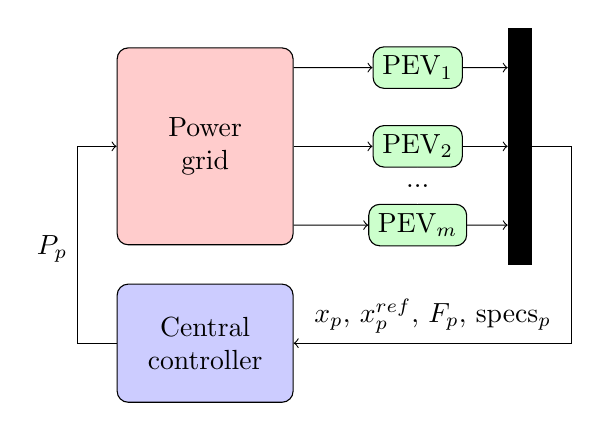
\begin{tikzpicture}[node distance=1.5cm]
        \node (grid) [draw, rectangle, text width=2cm, minimum height=2.5cm, align=center, fill=red!20, rounded corners] {Power \\grid};

        \node (pev2) [draw, rectangle, right of=grid, xshift=1.2cm, fill=green!20, rounded corners] {PEV$_2$};
        \node (pev1) [draw, rectangle, above of=pev2, yshift=-0.5cm, fill=green!20, rounded corners] {PEV$_1$};
        \node (pevm) [draw, rectangle, below of=pev2, yshift=0.5cm, fill=green!20, rounded corners] {PEV$_m$};

        \node (demux) [draw, rectangle, minimum width=0.3cm, minimum height=3cm, fill=black, right of=pev2, xshift=-0.2cm] {};

        \node (cc) [draw, rectangle, text width=2cm, minimum height=1.5cm, below of=grid, align=center, yshift=-1cm, fill=blue!20, rounded corners] {Central \\controller};

        \draw [->] ([yshift=1cm]grid.east) -- node[above] {\Lightning} (pev1.west);
        \draw [->] (grid.east) -- node[above] {\Lightning} (pev2.west);
        \draw [->] ([yshift=-1cm]grid.east) -- node[above] {\Lightning} (pevm.west);

        \draw [->] (pev1.east) -- ([yshift=1cm]demux.west);
        \draw [->] (pev2.east) -- (demux.west);
        \draw [->] (pevm.east) -- ([yshift=-1cm]demux.west);

        \draw [draw=white] (pev2) -- node[midway] {...} (pevm);

        \draw [->] (demux.east) -| ([xshift=0.5cm]demux.east) |- node[pos=0.75, above] {$x_p$, $x^{ref}_p$, $F_p$, specs$_p$} (cc.east);
        \draw [->] (cc.west) -| node[pos=0.74, left] {$P_p$}([xshift=-0.5cm]grid.west) -- (grid);
    \end{tikzpicture}
    \caption{Centralized approach block scheme.}
    \label{fig:cen_scheme}
\end{figure}